
\chapter{Ugeopgave 7}
\label{cha:ugeopgave-7}

\section{Del 1}

Vi har lavet et program der tegner et r�dt polygon og kaster en skygge i XwZw planet som kan ses p� figur \ref{fig:7-1-1}.

\begin{figure}[hp]
\centering
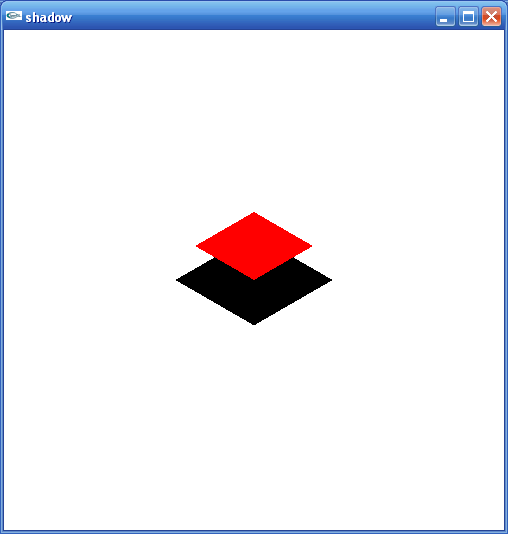
\includegraphics[width=8cm]{../exercise7/screenshots/1a.png}
\caption{Skygge i XwZw-planet}
\label{fig:7-1-1}
\end{figure}

Dern�st skulle skyggen flyttes ned i $Yw=-4$.
Vores l�sning flytter blot kassen og lyset 4 h�jere, da dette var en lettere l�sning. Resultatet kan ses af figur \ref{fig:7-1-2}.

\begin{figure}[hp]
\centering
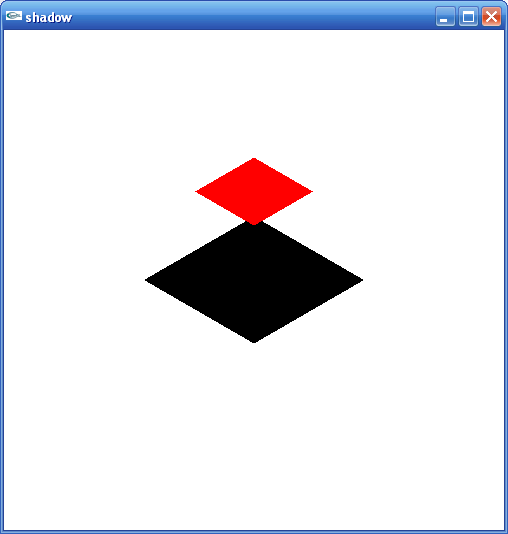
\includegraphics[width=8cm]{../exercise7/screenshots/1b.png}
\caption{Skygge i Yw = -4}
\label{fig:7-1-2}
\end{figure}

\section{Del 2}

Vi kunne tegne kassen med \texttt{glutSolidCube}, men har istedet valgt manuelt at lave alle koordinaterne til vertexerne for at pr�ve det.

Kassen kan ses p� figur \ref{fig:7-2-1} med dens tilh�rende skygge i YwZw planet hvor $Xw=-4$.

\begin{figure}[hp]
\centering
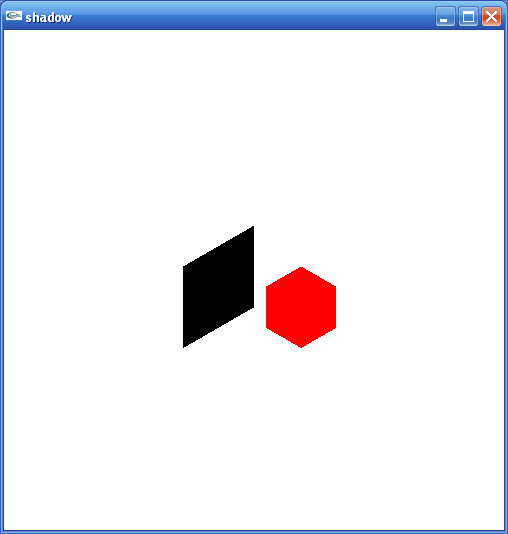
\includegraphics[width=8cm]{../exercise7/screenshots/2.png}
\caption{Cube}
\label{fig:7-2-1}
\end{figure}

\section{Del 3}

I denne delopgave skal der tilf�jes ``directional light'' til de to
foreg�ende opgaver. Det g�res ved at lave matricen $\mathbf{M}$ om til
at inkludere planet hvilket bla. ses ved l�sning af opgave 5.17\footnote{Angel s. 287}.

\begin{align*}
  \mathbf{M} = &
    \begin{bmatrix}
b \cdot d_y+c \cdot d_z & -b \cdot d_x & -c \cdot d_x & -d \cdot d_x\\
-a \cdot d_y & a \cdot d_x+c \cdot dz & -c \cdot d_y & -d \cdot d_y\\
-a \cdot d_z & -b \cdot d_z & a \cdot d_x+b \cdot d_y & -d \cdot d_z\\
0 & 0 & 0 & a \cdot d_x+b \cdot d_y+c \cdot d_z
    \end{bmatrix}
\end{align*}

Resultatet kan ses i figur \ref{fig:7-3-1}, \ref{fig:7-3-2} og \ref{fig:7-3-3}.

\begin{figure}[hp]
\centering
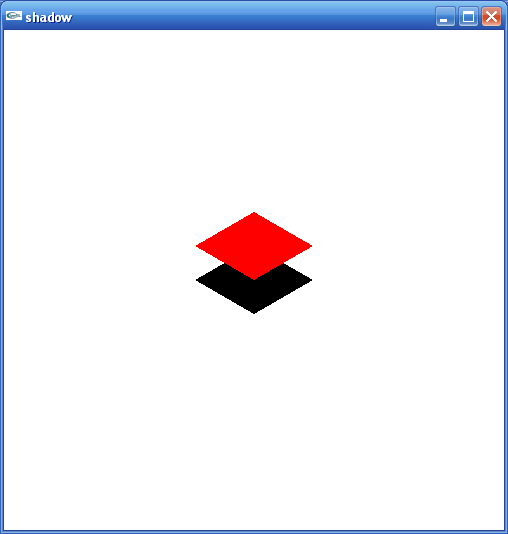
\includegraphics[width=8cm]{../exercise7/screenshots/3a.png}
\caption{Directional light}
\label{fig:7-3-1}
\end{figure}

\begin{figure}[hp]
\centering
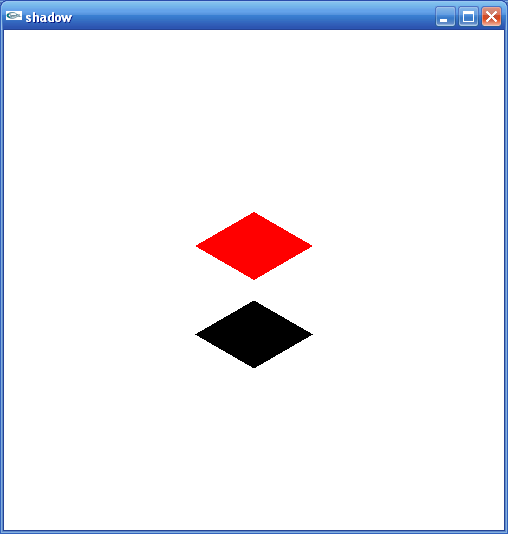
\includegraphics[width=8cm]{../exercise7/screenshots/3b.png}
\caption{Directional light i -4}
\label{fig:7-3-2}
\end{figure}


\begin{figure}[hp]
\centering
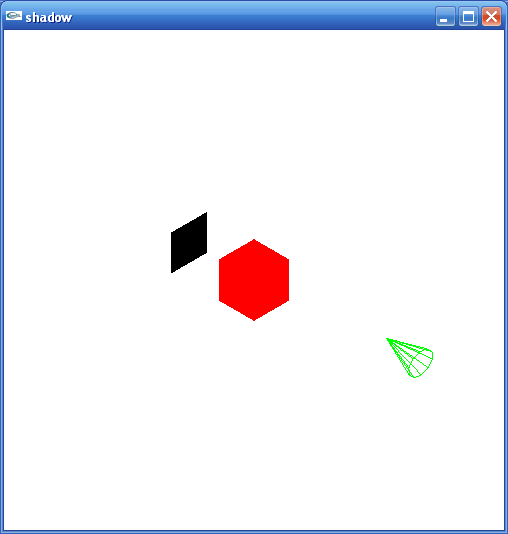
\includegraphics[width=8cm]{../exercise7/screenshots/3c.png}
\caption{Directional light p� kassen}
\label{fig:7-3-3}
\end{figure}

\section{Part 4}

Et andet eksempel p� kassen kan ses i figur \ref{fig:7-4-1}.

\begin{figure}[hp]
\centering
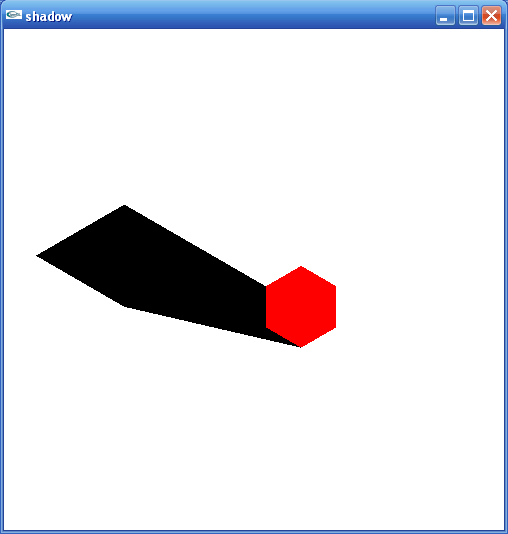
\includegraphics[width=8cm]{../exercise7/screenshots/4.png}
\caption{En anden belysning}
\label{fig:7-4-1}
\end{figure}